% !TEX root = /Users/zhuzhuangdi/Desktop/MSUCourses/MachineLearning847/17Project/17spr_wang_zhu_du/Middle/middle_report.tex
\section{Project Milestones}

\subsection{Completed Milestones}
%
\subsubsection{Background Survey}
% For this initial step, we plan to search for related works to computational literary creation to gain the basic knowledge of Song Ci.
%
We conducted large amount of survey on the state of the art approaches of SongCi generation. 
%
We find that this task attracts many interests both from the Natural Language Processing area and Machine Learning area. 
%
The approaches can be generalized into two kinds:  We either specify the generation rules (using templates), or build a model which can learn these rules automatically ( using neural network).
%
We also implemented some of the approaches proposed in previous work.
% 
% 
%
\subsubsection {Corpus Search and Analysis}
%
The dataset we use contains 18668 Ci, which contains a total number of 1183 poets and 1170 Pai. This dataset basically covers Ci generated during the entire Song Dynasty and the beginning of Yuan Dynasty. We analyze the number of poems wrote by each poet, which shown in Figure \ref{fig:poet}. Most of the poems are created by the first poets. The one that creates the most poems is Qiji Xin, one of the most famous poet of the Southern Song Dynasty. His poems covers a wide range of styles. Among all those poems, the bold style is most will known by now. In addition, we statistic the Pai of each poem. Ci was first used as a lyric, and Pai is the name of the tune. Each Pai has a specific melody and rhythm, so Ci has a fixed format requirements, such as the number of sentences, the number of words per sentence, pronunciation of those words, rhyme and so on. The statistical result is shown in Figure \ref{fig:Pai}. The most popular Pai is Silk-Washing Stream, followed by Prelude To Water Melody, Partridge Sky, Pusaman and River of Red. And there is good reason to believe that the songs that corresponding to these Pai are beautiful in melody, lively in rhythm and easy to sung, which caused them to be so popular in ancient China.
\begin{figure}[htbp]
	\centering
	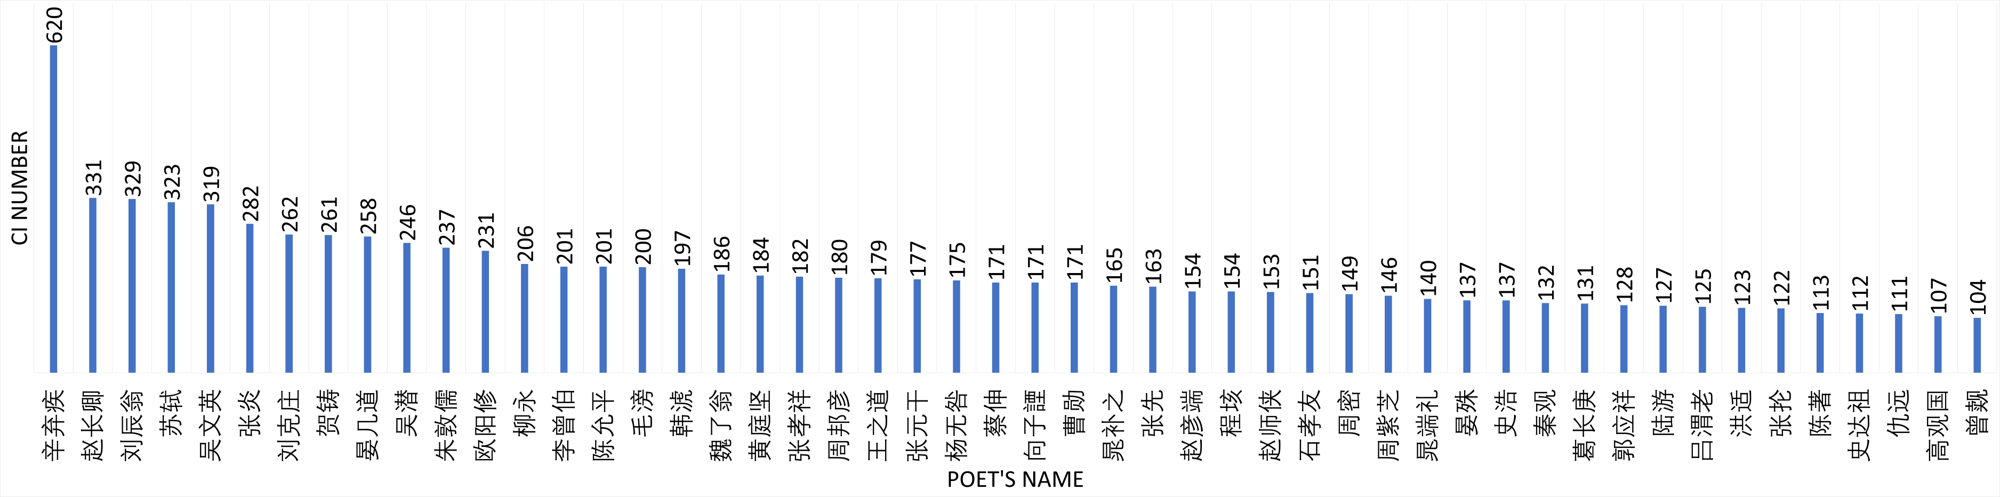
\includegraphics[width=0.9\linewidth]{poets.png}
	\caption{Poem Number Created by Top 50 Productive Poets}
	\label{fig:poet}
\end{figure}

\begin{figure}[htbp]
	\centering
	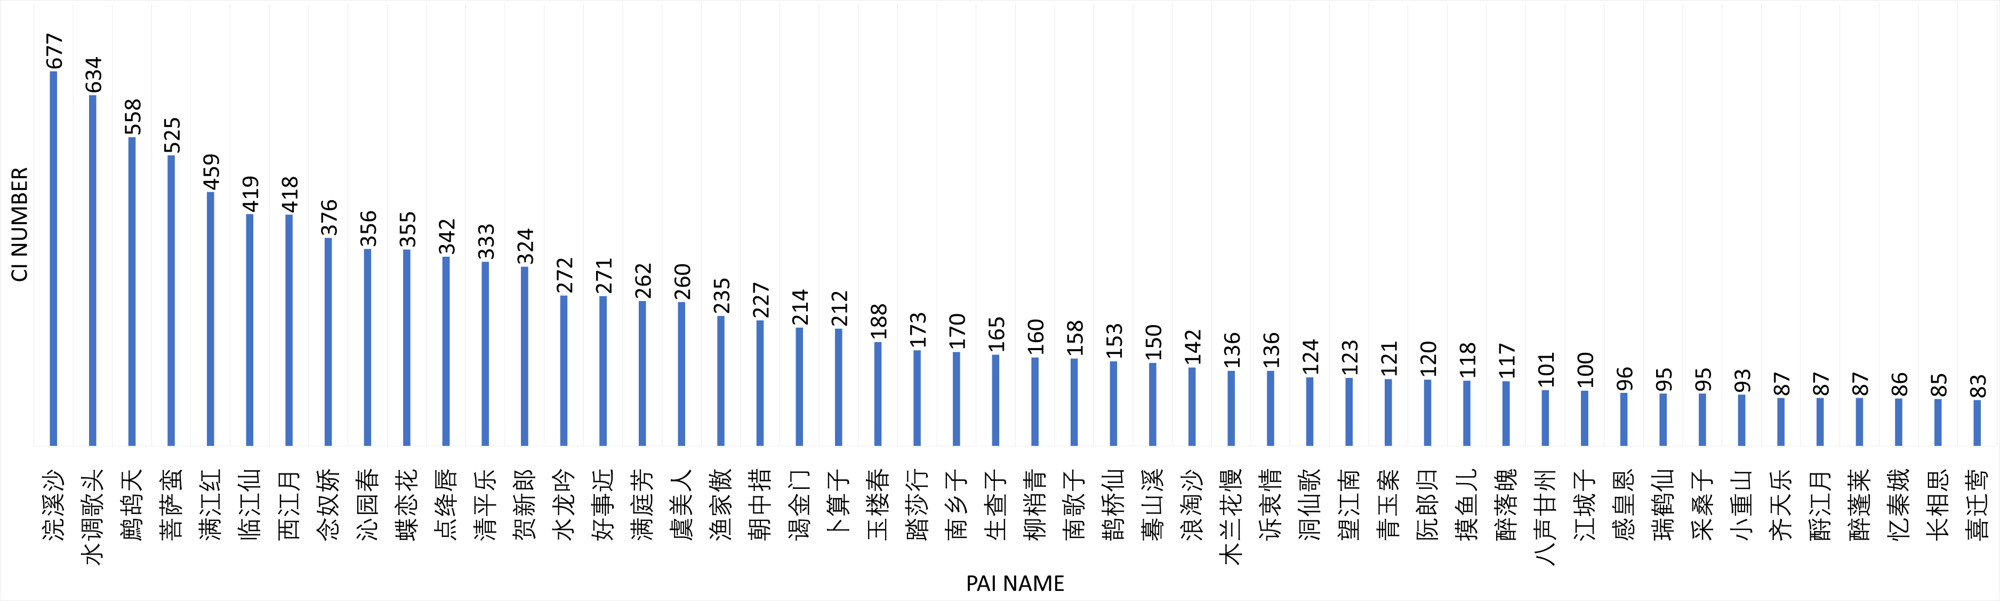
\includegraphics[width=0.9\linewidth]{Pai.png}
	\caption{Poem Number of Top 50 Popular Pai}
	\label{fig:pai}
\end{figure}
%

Word frequency analysis is to statistic and analyze the number of important words in the text, which is an important method of text mining. It is a traditional and useful content analysis method. The basic principle is to determine the overall style and theme of the entire article by the frequency of the words. By analyzing the word frequency in the poems, we have a general understanding of the style of poems and the process of writing those the poem, which can help us get more familiar with the grammar rules and themes of Ci. The most commonly used words can reveal common theme of Ci and the corresponding feelings. For example, we analyzed word frequency of season in our database. The result is shown in Figure \ref{fig:season}. We found that spring related words reached 2606, these words appeared in our dataset for 9210 times. Followed by autumn, there are 1167 words associated with autumn and appeared 3992 times. The unique scene in spring and autumn can trigger people's emotions, which might be the reason that so many poems are related with these two seasons.
\begin{figure}[htbp]
	\centering
	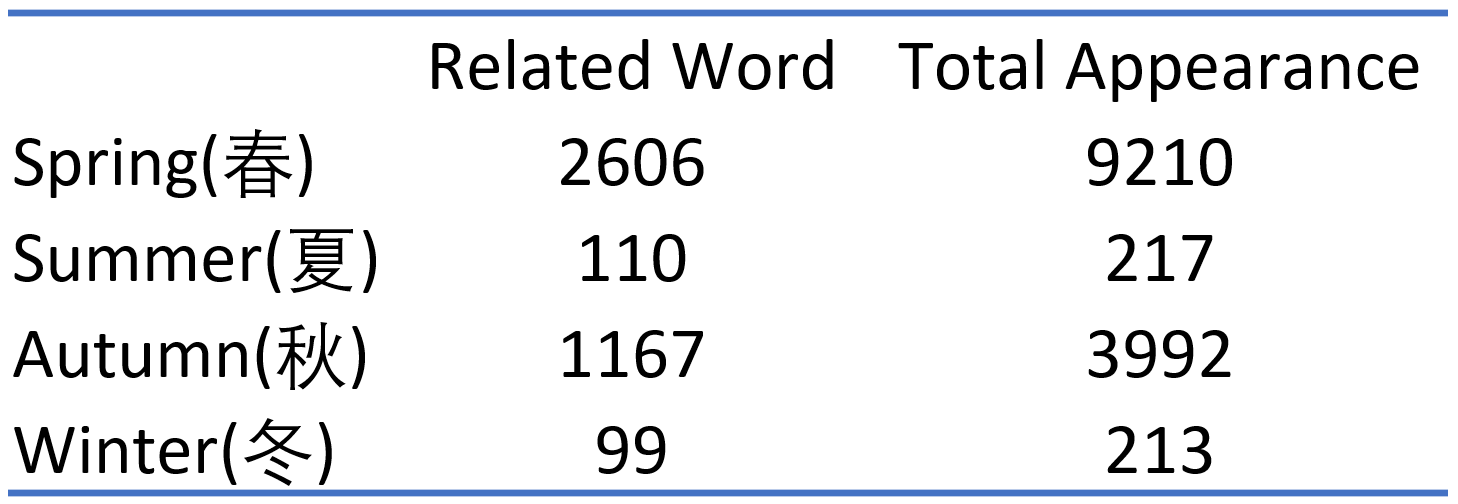
\includegraphics[width=0.8\linewidth]{season.png}
	\caption{Statistical Data of Season Related Word Frequency in Dataset}
	\label{fig:season}
\end{figure}
%
From most frequently used words, shown in Figure \ref{fig:wordcloud}, we found that the moon, east wind, mortal world, wine, dream, rain, flowers , sunset, old friends are the most commonly used images. Commonly used places, including Jiangnan, West Lake, Changan, Fairy Isle, Yangzhou. Commonly used verbs including laugh , come back, go back, lovesickness, look back, meet by chance. Commonly used emotions are hate, worry, hard, sigh, desolate, haggard. These words represent a very broad theme and style of Ci, including the description of leaving and missing, pride and enthusiasm, seasonal terms, chanting things, chanting nostalgia and so on.
\begin{figure}[htbp]
	\centering
	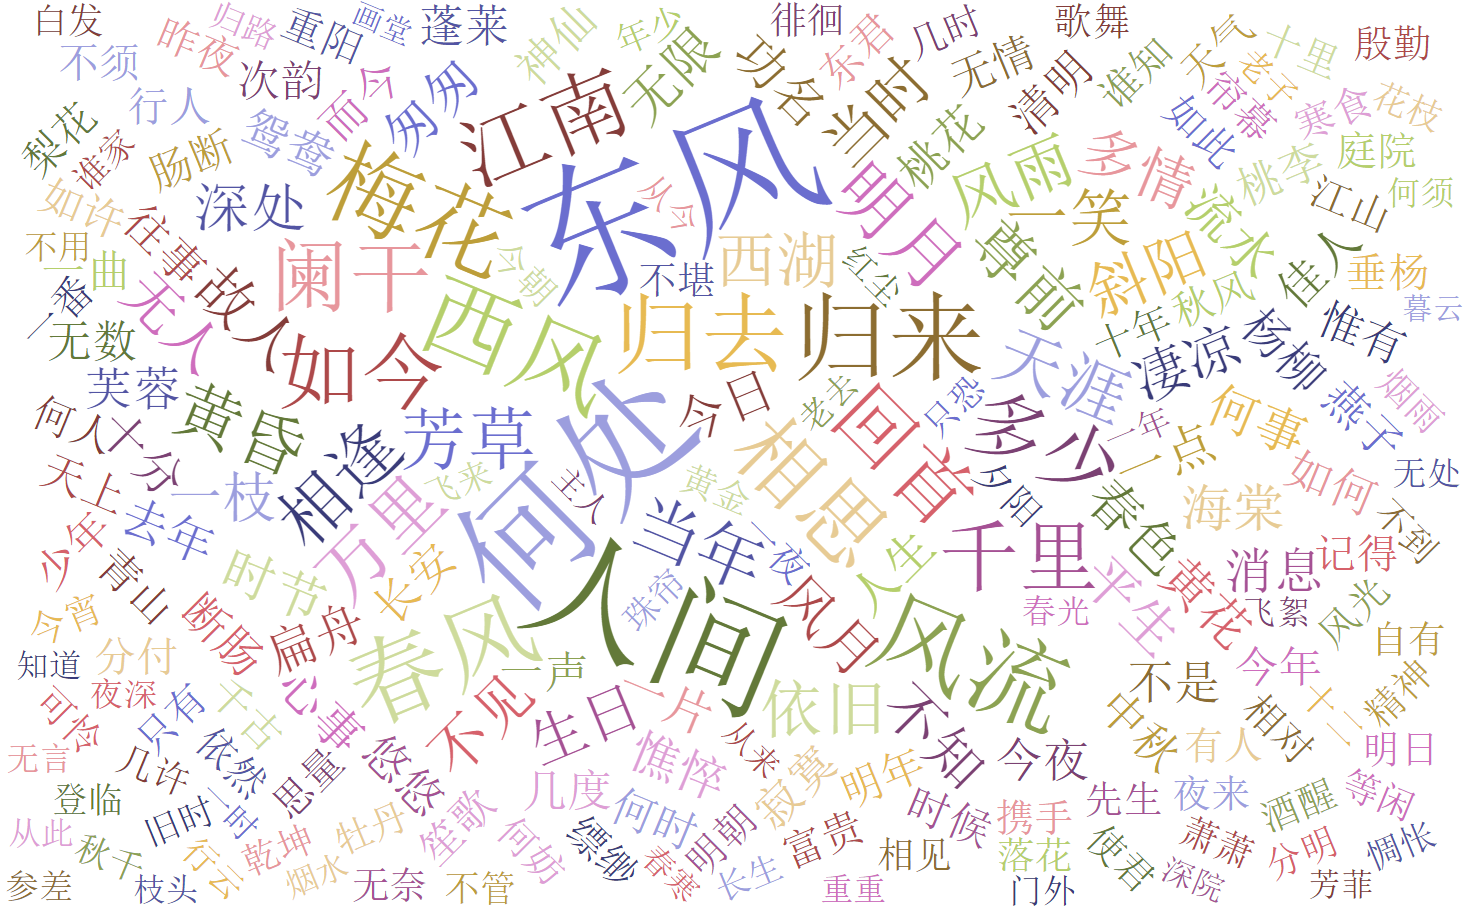
\includegraphics[width=0.9\linewidth]{wordcloud.png}
	\caption{Wordcould of Frequently Used Words in Dataset}
	\label{fig:wordcould}
\end{figure}
%
\subsubsection{ Implementation of a Vector Space Model }
Vector space models (VSMs) represent words in a continuous vector space where semantically similar words are mapped to nearby points.
%
We implemented this model to find the semantic relations between each Chinese character, so that given a few of keyword characters, such as 'spring' and 'beauty', we can generate poetries with coherent meanings using characters which are close to these keywords in the vector space.
%
%We use a predictive method to implement this  model based on the TensorFlow programming package \cite{tensorflow}.
%
We give a visualized result in Figure \ref{fig:VSM}. The figure is embeded with 100 Chinese characters in a 2-D space, which are randomly chosen from the most frequent 500 Chinese characters in the Song Ci corpus. The 2-D space corresponds to the first two dimensions in the vector space. We can see that words such as `spring', `sunny', and `breeze' are very close in the 2-D space, which convey similar sentimental feelings to readers. 


\begin{figure}[htbp]
	\centering
	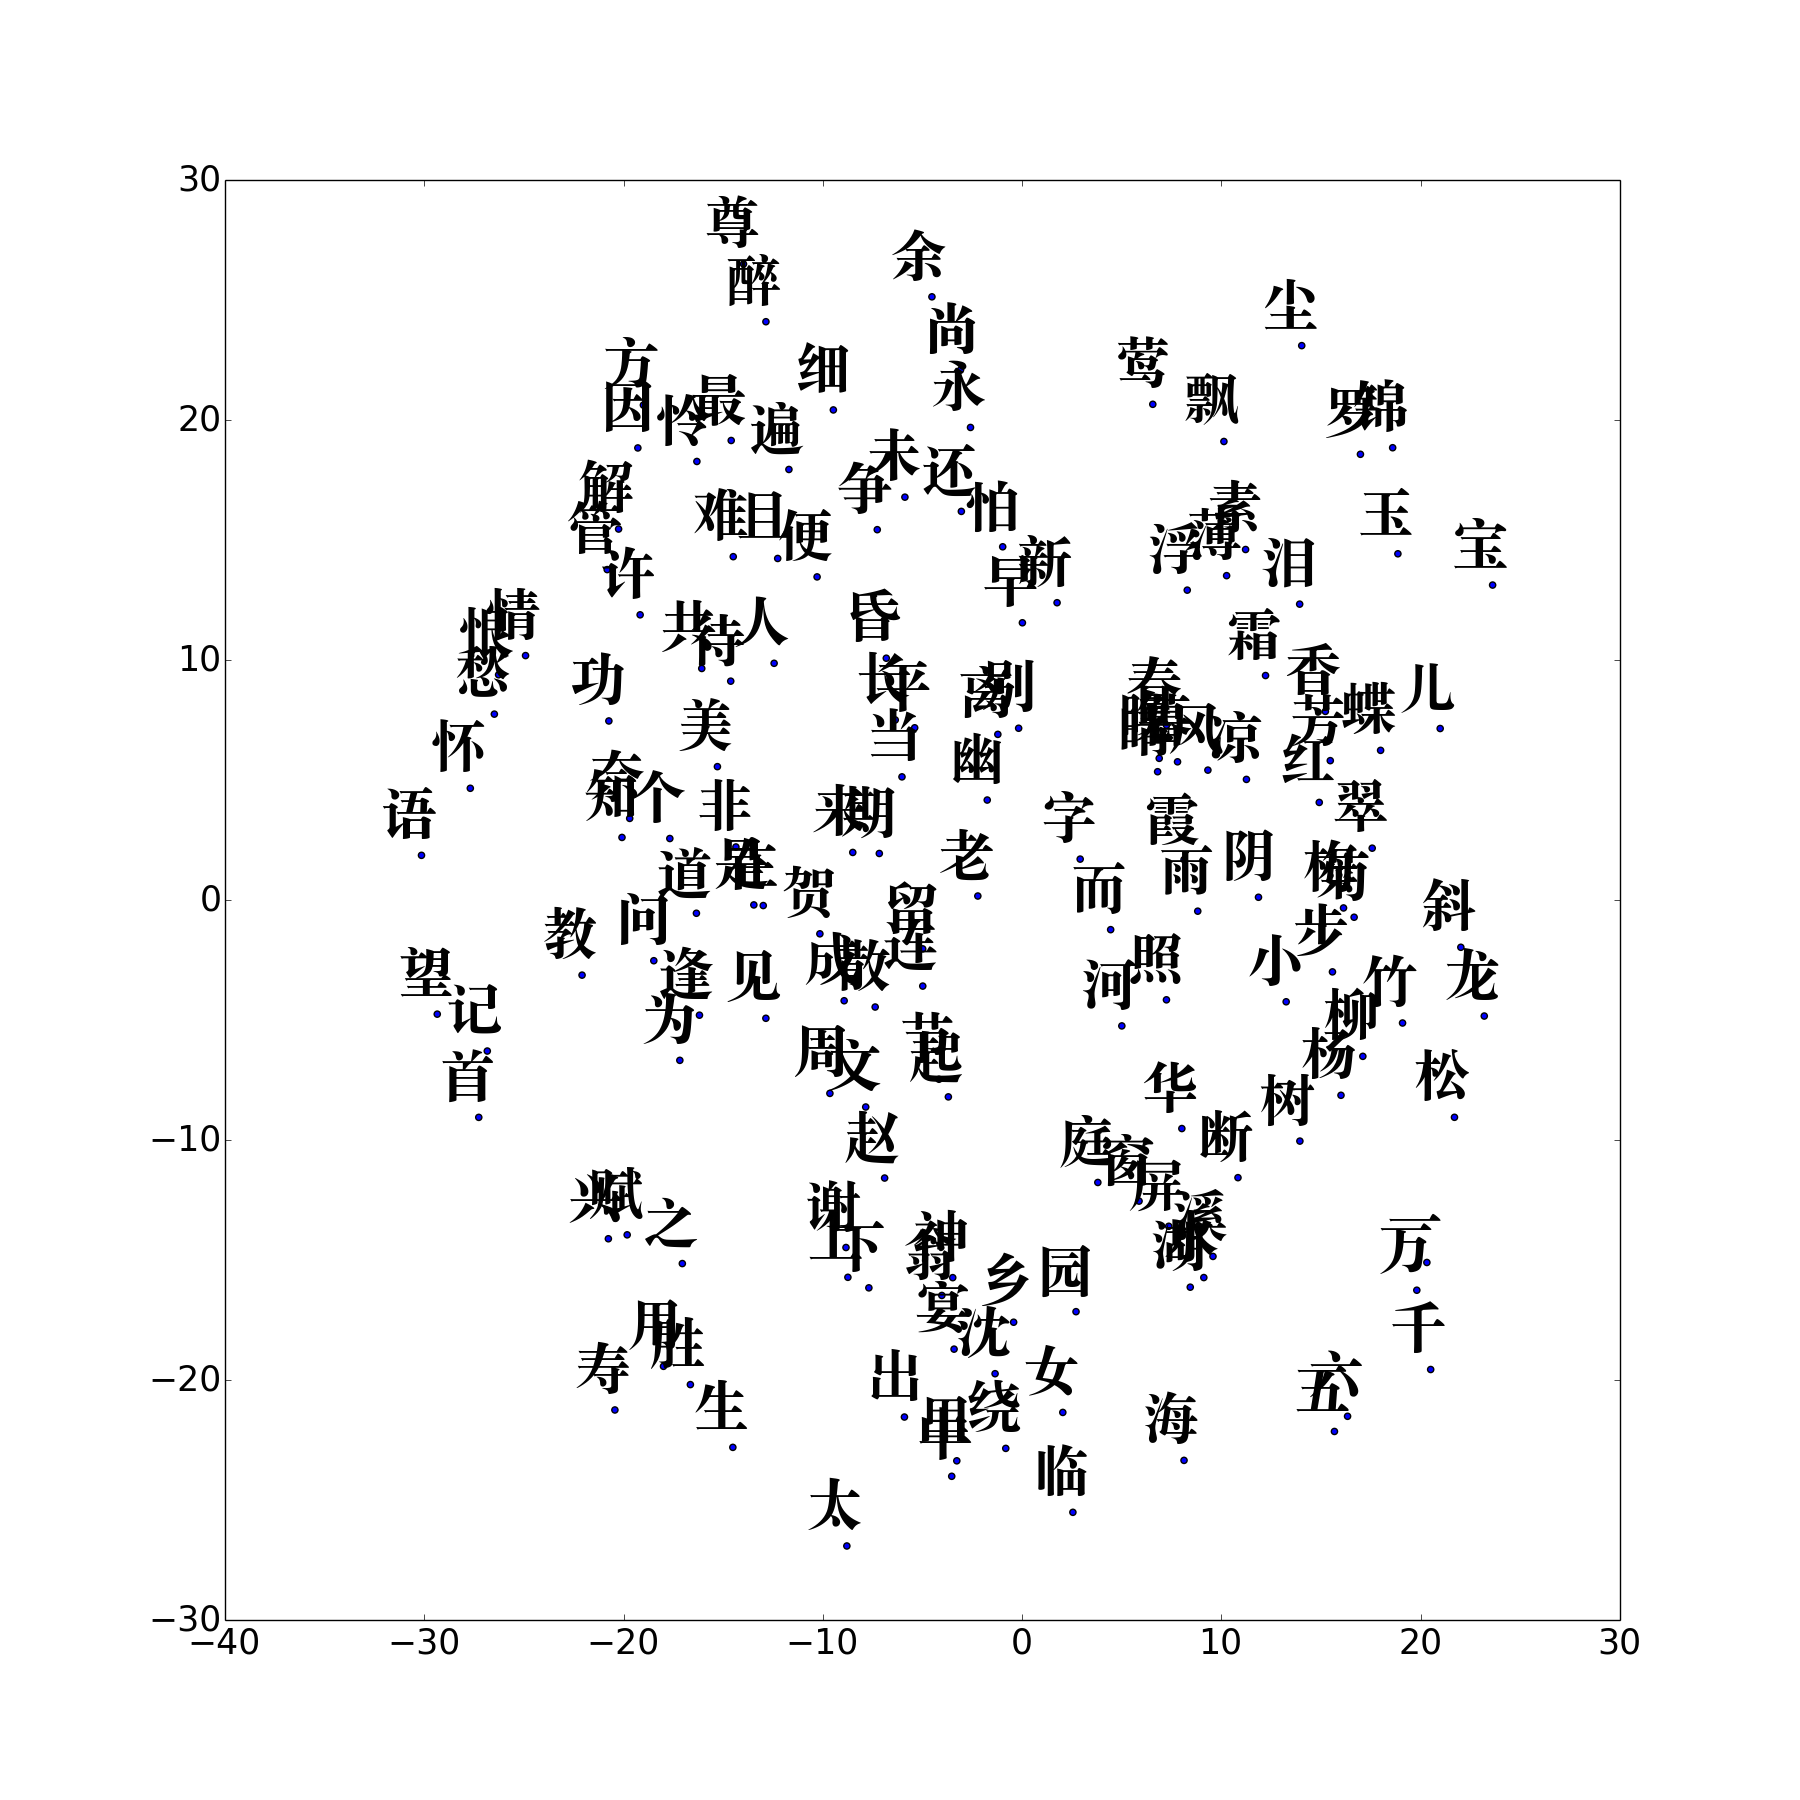
\includegraphics[width=0.9\linewidth]{tsne.png}
	\caption{Vector Space Model}
	\label{fig:VSM}
\end{figure}
\subsubsection{ Implementation of a RNN + LSTM Model  }
We implement a preliminary version of our model. It is a RNN model with Long Short Term Memory units (LSTM), which can capture long-term dependencies. 
%
We used deep learning packages called \emph{TensorFlow} \cite{tensorflow} to implement our model. The code is written in Python.
%
We present a preliminary result in Figure \ref{fig:poetry}, which is a quatrain poem. We can see that the poem conveys a feeling: the loneliness during travel. 


\begin{figure}[htbp]
	\centering
	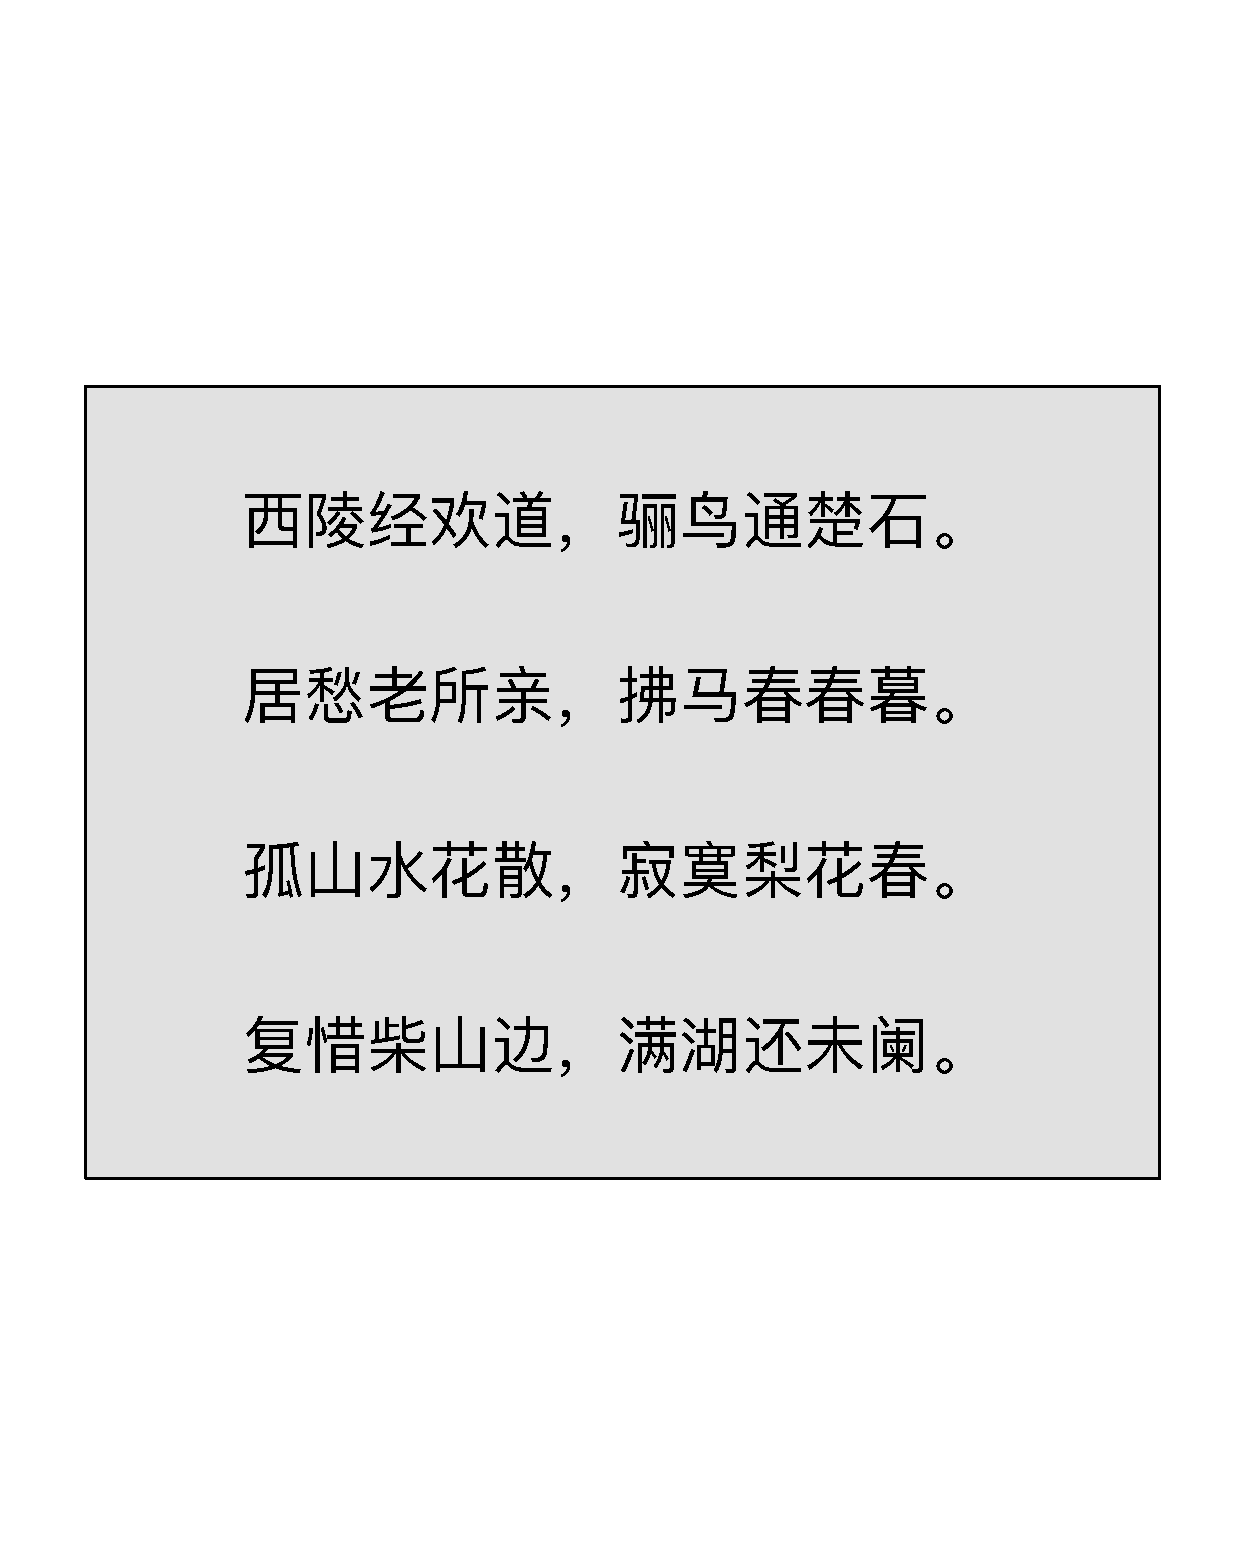
\includegraphics[width=0.5\linewidth]{poetry}
	\caption{A quatrain poem generated using RNN+LSTM model}
	\label{fig:poetry}
\end{figure}


\subsection{Remaining Milestones}
%
\subsubsection{Implementation of Song Ci Generating Model }
We used the Tang poetry corpus to train our model so the generated poem looks more like Tang poem than Song Ci. 
%
In our next step, we will explore the Song Ci dataset and focus on generating Song Ci poems.
%
We will continue to explore approaches to improve the performance of our model.

\subsubsection{Model Testing and Comparison}
We plan to use the valuation tools BLEU \cite{papineni2002bleu} to analyze the performance of the model. We will also compare the performance of our model with models proposed by state-of-the-art approaches.
\subsubsection{Project Writing} We will start on writting our project as we conduct the performance evaluation step. We plan to spend one week on the writting.



